%%%%%%%%%%%%%%%%%%%%%%%%%%%%%%%%%%%%%%%%%%%%%%%%%%%%%%%%%%%%%%%%%%%%%%%%%%%%%%%%%%%%
% Document data
%%%%%%%%%%%%%%%%%%%%%%%%%%%%%%%%%%%%%%%%%%%%%%%%%%%%%%%%%%%%%%%%%%%%%%%%%%%%%%%%%%%%
\documentclass[12pt]{article} %report allows for chapters
%%%%%%%%%%%%%%%%%%%%%%%%%%%%%%%%%%%%%%%%%%%%%%%%%%%%%%%%%%%%%%%%%%%%%%%%%%%%%%%%%%%%
\usepackage{preamble}

\begin{document}

\begin{center}
   \textsc{\large MATH 272, Homework 9, \emph{Solutions}}\\
\end{center}
\vspace{.5cm}

\newpage
\begin{problem}
	Let $\Psi(x)$ be a complex function with domain $[0,L]$.  Show that multiplication by a global phase $e^{i\theta}$ does not affect the norm of $\Psi(x)$ under the Hermitian (integral) inner product. In more generality, this shows that you cannot fully determine a quantum state -- there will always be an undetermined phase.
\end{problem}
\begin{solution}
	We take the following
	\begin{align*}
		\|e^{i\theta} \Psi\|^2=\innprod{e^{i\theta}\Psi}{e^{i\theta}\Psi} &= \int_0^L \left(e^{i\theta}\Psi(x)\right)\left(e^{i\theta}\Psi(x)\right)^*dx\\
		&= \int_0^L e^{i\theta}e^{-i\theta} \Psi(x)\Psi^*(x)dx\\
		&= \int_0^L \Psi(x)\Psi^*(x)dx\\
		&= \innprod{\Psi}{\Psi}\\
		&= \|\Psi\|^2.
	\end{align*}
\end{solution}

\newpage
\begin{problem}
	Consider the real function $f(x)=1$ on the domain $[0,L]$.
	\begin{enumerate}[(a)]
		\item What is the norm of $f$, $\|f\|$?
		\item Normalize $f(x)$.
		\item Find a nonzero normalized polynomial of degree $\leq 1$ that is orthogonal to $f(x)$.
	\end{enumerate}
\end{problem}
\begin{solution}~
	\begin{enumerate}[(a)]
		\item We compute the norm by
		\begin{align*}
			\|f\| = \sqrt{\innprod{f}{f}} &=\sqrt{ \int_0^L f^2(x)dx}\\
			&=\sqrt{ \int_0^L 1 dx}\\
			&= \sqrt{L}.
		\end{align*}
		\item We can normalize $f$ by letting $c$ be some constant and forcing
		\[
		1=\|cf\| = c^2L.
		\]
		Thus $c=\frac{1}{\sqrt{L}}$.  We can write the normalized function as
		\[
		h(x)=\frac{1}{\sqrt{L}}. 
		\]
		\item Consider an arbitrary polynomial of degree $\leq 1$ by putting $g(x)=ax+b$.  Now, we want this polynomial to be orthogonal to $f(x)$ which means that we want
		\[
		\innprod{f}{g}=0.
		\]
		Let us compute the above
		\begin{align*}
			\innprod{f}{g} &= \int_0^L f(x)g(x)dx\\
			&=\int_0^L ax+bdx\\
			&= \frac{aL^2}{2}+bL\\
			&= \frac{1}{2}L\left(aL+2b\right).
		\end{align*}
		Hence, we can solve for $a$ by
		\[
		0=aL+2b \quad \implies \quad a= -\frac{2b}{L}.
		\]
		Now, $g(x)=-\frac{2b}{L}x+b$.  But, we require $g(x)$ to be normalized as well hence
		\begin{align*}
			1=\innprod{g}{g} &= \int_0^L \left(-\frac{2b}{L}x+b\right)^2dx\\
			&= \frac{b^2L}{3}.
		\end{align*}
		Solving for $b$, we find $b=\sqrt{\frac{3}{L}}$ and hence we have that
		\[
		g(x) = -2\sqrt{\frac{3}{L^3}}x+\sqrt{\frac{3}{L}}..
		\]
	\end{enumerate}
\end{solution}

\newpage
\begin{problem}
	A wavefunction $\Psi(x)$ for a particle in the 1-dimensional box $[0,L]$ could be written as a superposition of normalized states
	\[
	\psi_n(x) = \sqrt{\frac{2}{L}} \sin\left(\frac{n\pi x}{L}\right).
	\]
	That is,
	\[
	\Psi(x) = \sum_{n=1}^\infty a_n \psi_n(x),
	\]
	for some choice of the coefficients $a_n$.
	\begin{enumerate}[(a)]
		\item Let $a_n = \frac{\sqrt{6}}{n\pi}$. Show that $\Psi(x)$ is normalized. \emph{Hint: first, use orthogonality of the states $\psi_n(x)$ to your advantage. Then you will need to know what an infinite series evaluates to. Use a tool like WolframAlpha to evaluate this series.}
		\item Note that we can approximate $\Psi(x)$ by taking a finite sum approximation up to some chosen $N$ by
		\[
			\Psi(x) \approx \sum_{n=1}^N a_n \psi_n(x).
		\]
		Plot the approximation of $\Psi(x)$ for $N=1,5,50,100$.  \emph{Hint: you can modify my Desmos examples.}
		\end{enumerate}
\end{problem}
\begin{solution}
	\begin{enumerate}[(a)]
		\item To see that $\Psi(x)$ is normalized we take
		\begin{align*}
			\innprod{\Psi}{\Psi} &= \innprod{\sum_{n=1}^\infty a_n \psi_n(x)}{\sum_{n=1}^\infty a_n \psi_n(x)}\\
			&= \sum_{n=1}^\infty \|a_n\|^2 \innprod{\psi_n}{\psi_n} &\textrm{by orthogonality of the states}\\
			&= \sum_{n=1}^\infty \frac{6}{n^2 \pi^2}\\
			&= \frac{6}{\pi^2} \sum_{n=1}^\infty \frac{1}{n^2}\\
			&= \frac{6}{\pi^2} \zeta(2)\\
			&= 1.
		\end{align*}
		Note the sum above is the Zeta function we saw in Math 271 and $\zeta(2)$ is a well-known value (that you can find by computing the above sum in, for example, WolframAlpha.
		\item ~
	\begin{figure}[H]
	\centering
		\begin{subfigure}[h]{0.48\textwidth}
			\centering
			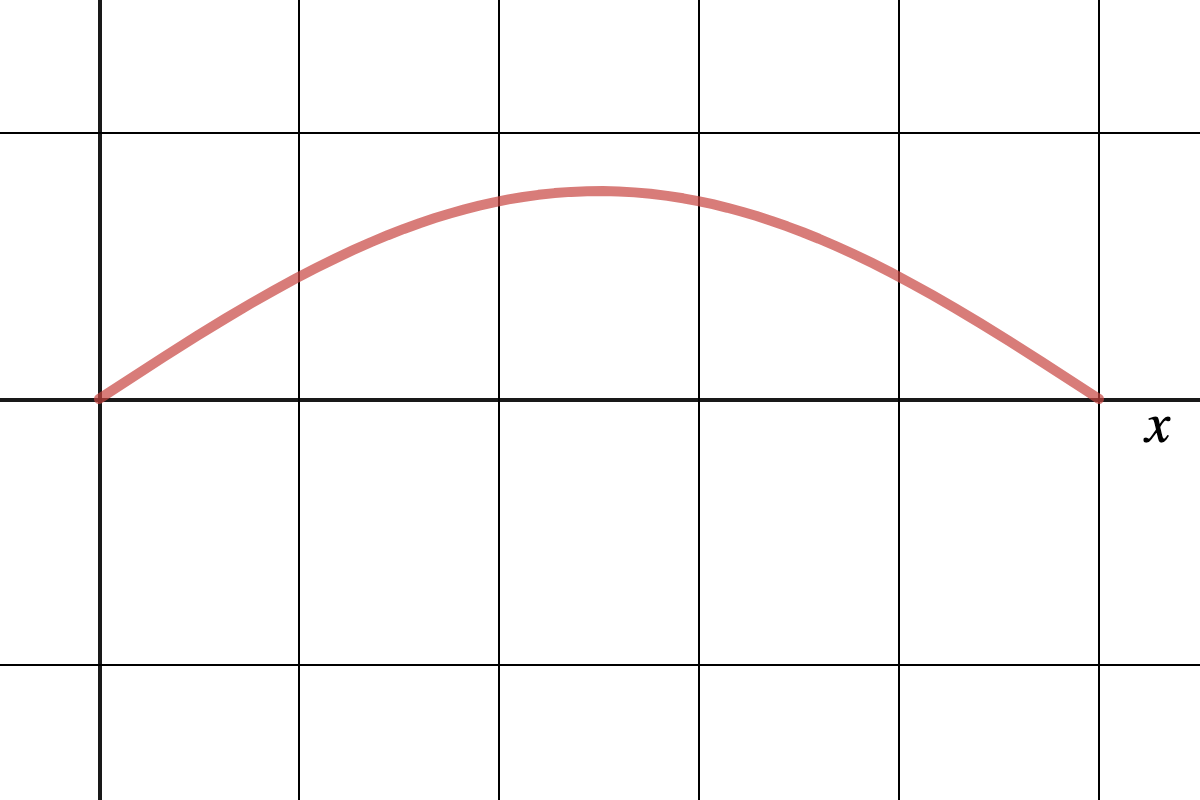
\includegraphics[width=.8\textwidth]{n=1.png}
			\caption{The approximation to $\Psi(x)$ with $N=1$.}
		\end{subfigure}
		~
		\begin{subfigure}[h]{0.48\textwidth}
			\centering
			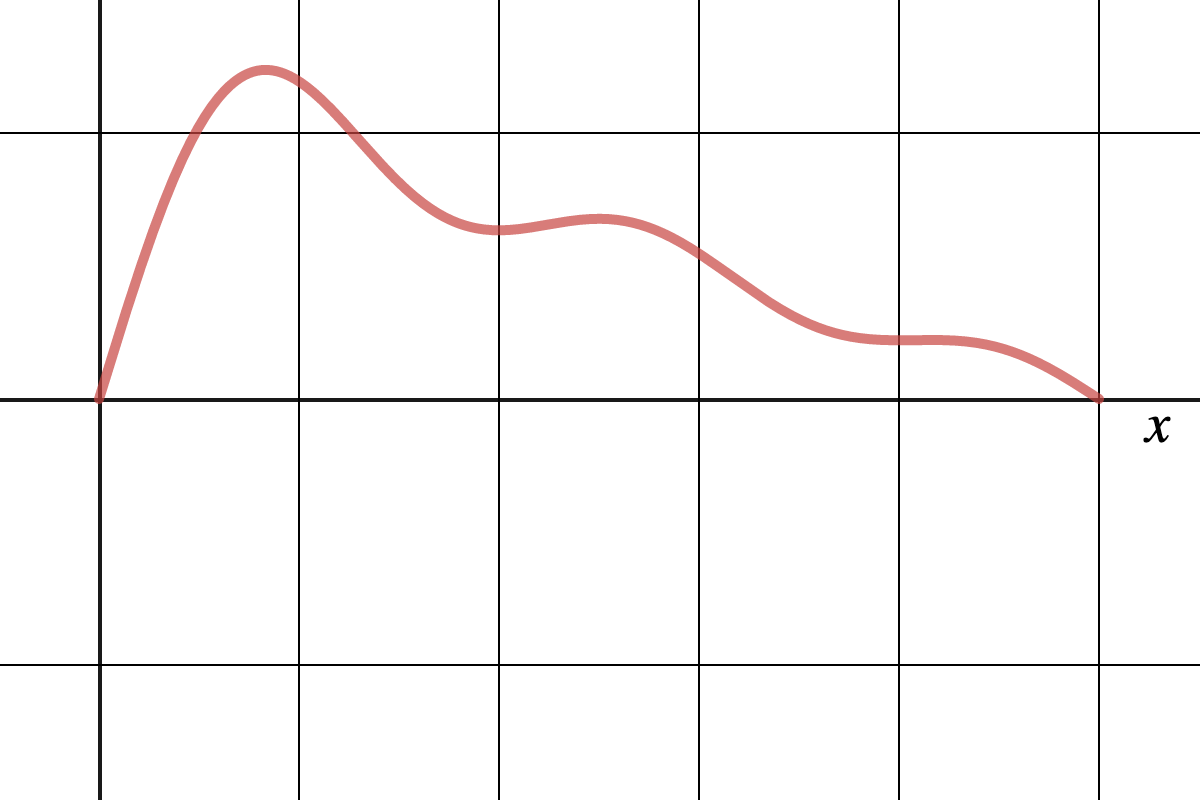
\includegraphics[width=.8\textwidth]{n=5.png}
			\caption{The approximation to $\Psi(x)$ with $N=5$.}
		\end{subfigure}
		\\
		\begin{subfigure}[h]{0.48\textwidth}
			\centering
			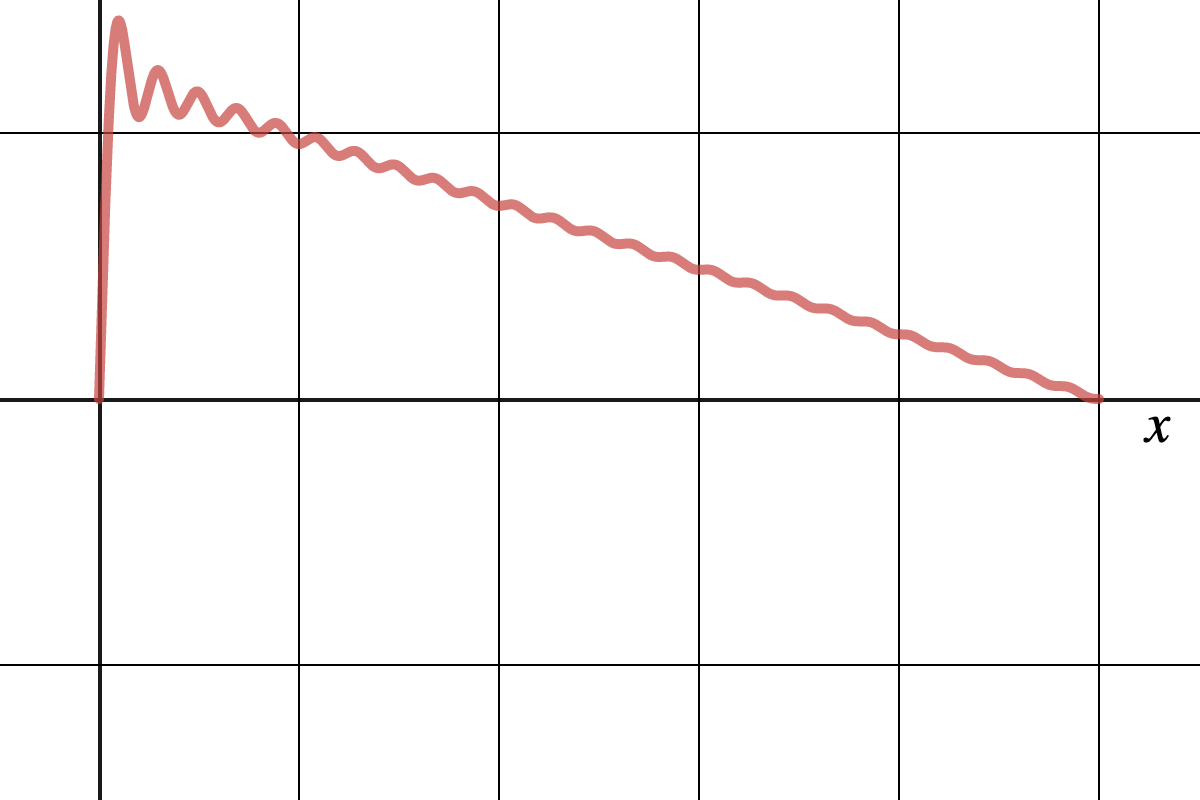
\includegraphics[width=.8\textwidth]{n=50.png}
			\caption{The approximation to $\Psi(x)$ with $N=50$.}
		\end{subfigure}
		~
		\begin{subfigure}[h]{0.48\textwidth}
			\centering
			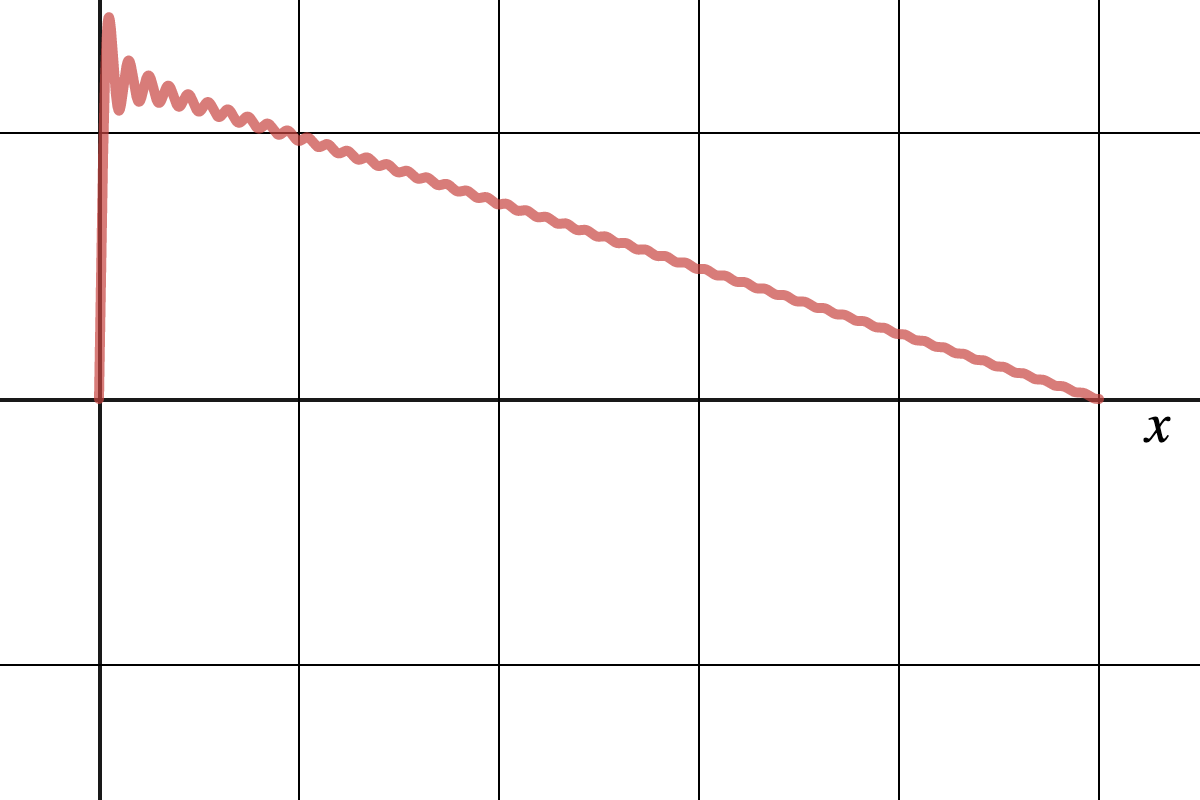
\includegraphics[width=.8\textwidth]{n=100.png}
			\caption{The approximation to $\Psi(x)$ with $N=100$.}
		\end{subfigure}
	\end{figure}
	\end{enumerate}
\end{solution}

%\newpage
%\begin{problem}
%	Suppose we have two vectors $\vecu,\vecv \in \R^3$.  We can compute the distance between the vectors
%	\[
%	d(\vecu,\vecv) = \|\vecu-\vecv\| = \sqrt{(\vecu-\vecv)\cdot(\vecu-\vecv)}.
%	\]
%	That is to say, we inherit not only a norm from an inner product, but a distance function from a norm!  Intuitively, we are finding the length (or norm) of the vector extending from the head of $\vecv$ to the head of $\vecu$.
%	\begin{enumerate}[(a)]
%		\item Show that
%		\[
%		d(\vecu,\vecv) = \sqrt{\|\vecu\|^2+\|\vecv\|^2-2\vecu\cdot \vecv}.
%		\]
%		\item Compute the distance between vectors $\vecu=\xhat + \zhat$ and $\vecv = \xhat - \yhat$.  
%		\item Extend this notion to compute the distance between the Legendre polynomials $f_1,f_2\colon [-1,1] \to \R$ where $f_1(x)=\sqrt{\frac{3}{2}}x$ and $f_2(x)=\sqrt{\frac{5}{8}}\left(1-3x^2\right)$. \emph{Hint: make sure you use the correct integral inner product for this domain!}
%	\end{enumerate}
%\end{problem}
%\begin{solution}~
%	\begin{enumerate}[(a)]
%		\item We take
%		\begin{align*}
%			d(\vecu,\vecv)&= \sqrt{(\vecu-\vecv)\cdot(\vecu-\vecv)}\\
%				&= \sqrt{\vecu\cdot \vecu + \vecu\cdot (-\vecv) + (-\vecv)\cdot \vecu +(-\vecv)\cdot (-\vecv)}\\
%				&= \sqrt{\|\vecu\|^2 + \|\vecv\|^2 -2\vecu \cdot \vecv}.
%		\end{align*}
%		\item Let us compute each part of the distance formula,
%		\[
%		\|\vecu\|= \sqrt{2}, \qquad \|\vecv\|=\sqrt{2}, \qquad \vecu \cdot \vecv = 1.
%		\]
%		Hence we have
%		\[
%		d(\vecu,\vecv) = \sqrt{2+2-2}=\sqrt{2}.
%		\]
%		\item In order to compute a distance between functions we can just replace the dot product with the Hermitian inner product in the form 
%		\[
%		\innprod{f}{g}=\int_{-1}^1 f(x)g(x)dx. 
%		\]
%		This then gives us an induced norm that we will use in replacement of the Euclidean norm above.  We now compute
%		\[
%		\|f_1\| = \int_{-1}^1 |f_1(x)|^2 dx = 1, \qquad \|f_2\|=\int_{-1}^1 |f_2(x)|^2dx =1, \qquad \innprod{f_1}{f_2} = \int_{-1}^1 f_1(x)f_2(x)dx =0.
%		\]
%		Thus we have the distance
%		\[
%		d(f_1,f_2) = \sqrt{1+1-0}=\sqrt{2}.
%		\]
%	\end{enumerate}
%\end{solution}









\end{document}